\chapter{Introduction and Approach}\label{Introduction and Approach}

% BEGIN Justin's section

The following report describes the work of the software team on the MCTX3420 pressurised can project during Semester 2, 2013 at UWA. The report is intended to assist others in comprehending the decisions and processes involved, as well providing a tool for further development of the system. The report serves as a record of the planning, design, coding, testing and integration of the system, with specific reference to the development of the system software. Extensive documentation is also provided via a project wiki\cite{mctx3420_wiki}.

The MCTX3420 project aimed to build an experimental apparatus for measuring the behaviour of a container with pressure --- in this case, testing how a drink can deformed as air pressure inside it increased. The desired result was a self-contained, safe, reliable, effective and easy-to-use system which could perform the desired experimental tasks, to be used by both students and wider industry professionals.

Unfortunately, the system is (as of 1st November 2013) still not complete; the hardware components have not been fully tested and integrated with the software, despite extensive work by all students. However, the project is very close to completion. The software can interact in the desired manner with the hardware components, and fulfils the majority of the required functionality. With some further testing and development using the final hardware, the software could easily be implemented --- and the report has been written with this in mind, allowing another group in the future to build upon the project software.

The report begins with an overview of the whole system and the design of the software component. Each subsection then focuses on a specific aspect of the software, going into detail about its design, development, functionality, testing, and integration. Following this, there are sections focusing on the administrative aspects of the project, including teamwork, the general development process, and costs. The report concludes with some documentation of the software and recommendations for future development.

\section{System Overview}

To aid understanding of the context of the software project, a brief overview of the system as a whole is presented below. Essentially, the MCTX3420 project apparatus is designed to test the behaviour of a pressure vessel as air pressure inside it is gradually increased. A very basic system diagram showing the main components is shown in Figure \ref{system_overview.png}, with control components in \textcolor{red}{ red}, electronics in \textcolor{green}{ green}, sensors in \textcolor{Purple}{ purple}, pneumatics in \textcolor{blue}{ blue}, and experimental targets in \textcolor{Orange}{ orange}.

\begin{figure}[H]
	\centering
	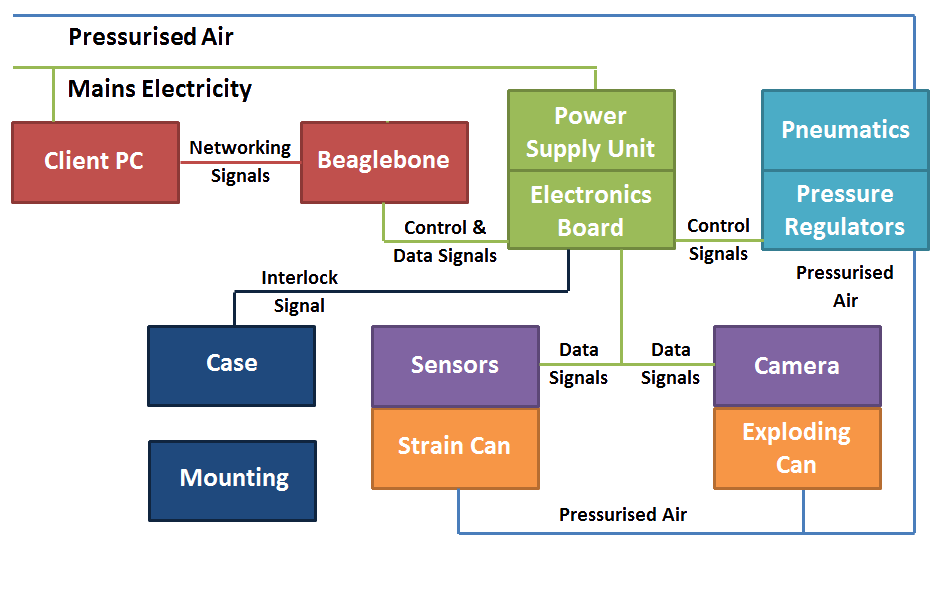
\includegraphics[width=0.8\textwidth]{figures/system_overview.png}
	\caption{Block diagram of the physical system} 
	\label{system_overview.png}
\end{figure}

\subsection{Experimental Procedure}

The general experimental procedure is to increase the pressure inside a pair of pressure vessels (in this case, drink cans), measuring one's deformation behaviour and measuring the other to failure point. The user does this by logging into a web browser interface, starting a new experiment, and increasing system pressure in the desired fashion.

As pressure is increased, the web browser passes this instruction to the system controller, which manipulates the pneumatic pressure regulators to input correct pressure to the measured can. While doing this, the system controller also reads from a collection of sensors and returns this data to the web browser (strain, pressure, dilatometer deformation, visual images). The vessel's deformation with pressure can then be characterised.

This continues until the desired final pressure is reached. Then, pressure in the failure can may be increased further until that can reaches its failure point. The experiment then ends and the system is returned to room pressure. The user can view and download the resulting data.

\subsection{Components}

The main areas of the system are as follows:

\begin{itemize}
	\item {\bf Control:} The experiment is controlled through web browser interface from a client PC. This web interface connects to a server running on what is effectively a small, integrated PC --- the ``BeagleBone Black'' --- and this server directly controls the experiment hardware and reads the sensor data, providing a low-level interface to the system's electronics. The BeagleBone itself is situated inside the experiment case, and the client PC connects to the BeagleBone server through the local network.
	\item {\bf Electronics:} Because the system features a large array of electronic components, these must be run through a central filtering and amplification system to ensure that correct voltages and currents are provided. There is a circuit board inside the case which performs this task. The board connects the BeagleBone, pneumatics, sensors, and power supply to facilitate system operation. System power is provided by a PSU connected to the mains.
	\item {\bf Pneumatics:} The system's pneumatics feed the desired air pressure into the two pressure vessels being tested. Air is fed through a series of pipes from the laboratory's pressurised air supply; solenoid valves control on/off air flow through the system, while pressure is controlled via regulators. Exhaust valves are provided for venting the system. Pneumatics are controlled by the BeagleBone, with signals fed through the electronics board.
	\item {\bf Sensors:} A suite of sensors is used to collect system data and measure the deformation of the pressure vessel. The sensors include strain gauges, pressure sensors, a microphone, a dilatometer/microscope, and a camera --- these give a comprehensive set of data to match the can's deformation to the pressure level. Each sensor has a different output and must be conditioned by the central electronics board before its data is recorded by the BeagleBone.

	\item {\bf Mounting and Case:} The mounting system for the cans uses a screw-in mechanism to achieve an airtight seal. This holds the can in place so that pressure can be fed into it through the base of the mount. The system case holds all of the components in a sealed protective compartment, which ensures that the system will be safe in the event of failure and physically separates the various systems. The case also features an interlock switch that prevents any operation of the system if the lid is not fastened.

\end{itemize}

The system software essentially is defined by the ``control'' component: allowing a user to control the experiment hardware. To do this, the software must successfully interface with all of the system areas above so that the desired experiment can be run. 

\section{Development Process}

The development process is outlined below. Each part of the software followed the same general process, which is discussed in more detail for each section later in the report.

\subsection{Planning and Design}
First, the actual software task to be completed is identified; this is organised with group input. The software component is then designed according to the requirements. Parameters and features are chosen based on the project guidelines and how the component interacts with other software. 

\subsection{Coding}

Each section is then actually written. Most of the initial work is done individually (for consistency) and completed in between meetings. At group meetings the code is presented, and may be edited by other team members to fix issues, increase efficiency, and integrate it with other code sections.


Extremely important to development was the use of the Git system\cite{github,gitucc} and GitHub website\cite{github}. GitHub is specially designed for software use and is essentially a web-based hosting service for development projects, which uses the Git revision control system. It allows all team members to contribute to the same project by working on their own local ``forks'', and then ``merging'' their changes back into the main branch of software\cite{github_fork}.

The Git system ensures that work by different team members is tracked\cite{github_contribs}, that work fits together consistently, and that other work is not accidentally overwritten or changed (important when dealing with large amounts of code). Git also features a notifications and issue tracking system with email alerts whenever a change is made. The basic GitHub process is as follows:

\begin{enumerate}
	\item Create an individual ``fork'' of the software, separate from the main branch.
	\item Modify this fork on a local machine with proposed changes or additions. This fork is also updated regularly with any changes that were made in the main branch.
	\item When work is complete, create a ``pull request'' to merge local changes back into the main code base.
	\item The pull request can be reviewed by other team members; if everything fits, the request is accepted and the local changes become part of the main code. 
\end{enumerate}
In this way, GitHub automates the more tedious aspects of code management.

Another important aspect of the coding process is coding style. Throughout the project, all code that was written adhered to the same style to make it consistent and easier to read. One aspect of styling, for example, is use of capitals when defining function names (for example, \funct{Actuator_Init}), variable names (\var{g_num_actuators}), or definitions of constants (\var{ACTUATORS_MAX}), to make it immediately clear whether something is a function, variable or constant. Other aspects include use of indentation, the ordering of functions, and frequent use of comments. Essentially, styling is used to ensure the code is consistent, easy to follow, and can therefore be worked on by multiple people. 

Coding style is also important when following general code standards. The C language features many standards and style guidelines which were also adhered to, to make the code readable by wider industry professionals. Some examples of this include beginning global variables with \texttt{g_} and correct use of brackets as separators\cite{mellon}. All efforts were made to follow common C and HTML code standards. The use of a common coding style and standards will hopefully make the project software easily expandable by others in the future.


Code was also expected to adhere to safety standards. In the first weeks of the project, a document\cite{kruger_safety} was created that outlined all aspects of software safety - both for the software design itself, and ensuring that the system was still safe if the software failed. The results of this are explained further later in the report, with one example being the server's ``sanity check'' functions.

\subsection{Testing}

Once the software section is relatively complete, it can be tested with the larger code base. This was generally done through writing specific test functions. Because the operating system on the BeagleBone (GNU/Linux) is widely available for commercial PCs and laptops, software development and testing could occur without needing to wait for a BeagleBone to become available. Code was also tested on the BeagleBone itself where possible to ensure correct operation. One example is for the sensors software - initially, functions were written that simulated sensors, so it could be tested if data was read correctly. These functions were rewritten for use with actual hardware as the specifics became known later in the project.

\subsection{Collaboration}
After the testing process is satisfied, the final code can be committed to the system. This requires input from the other project teams. If there is any feedback or the requirements change in the future, the code can be edited through the above process.

\section{Team Collaboration}

Collaboration between members of the software group was extremely important throughout the project. Members were often individually responsible for different areas of software --- or, alternately, were simultaneously rewriting different sections of the same code --- so it was essential to make sure that all parts were compatible, as well as completed on schedule. Communication between the software group and other project groups was similarly vital, to ensure that all work contributed to the project's end goals. 

\subsection{Communication} \label{Communication}
The primary time for collaboration was during the team's weekly meetings. Meetings occurred at 2pm-4pm on the Monday of every week, and were generally attended by all group members. While most work was expected to be done outside this time, the meetings were valuable for planning and scheduling purposes, for tackling problems and making design decisions as a group. Team members were able to work together in the meetings to complete certain tasks much more effectively. Importantly, at the end of each meeting, a report of the work done during the prior week and a list of tasks to do the following week was produced, giving the project a continuous, clear direction. 

GitHub was used as the group's repository for software work. The usefulness of GitHub was explained previously in the ``General Development Process'' section, but essentially, it is a very effective tool for managing and synchronising a large, multi-person software project. GitHub also features a notifications and issue-tracking system, which was useful for keeping track of tasks and immediately notifying team members of any changes.


Outside of meetings, email was the main form of communication. Email threads exist for all of the project's main areas, discussing any ideas, changes or explanations. Email was also used for announcements and to organise additional meetings. For less formal communication, the software group created their own IRC channel. This was essentially a chat channel that could be used to discuss any aspect of the project and for communication about current work.

\subsection{Scheduling}

At the beginning of the project, an overall software schedule was created, outlining the main tasks to be completed and their target dates. While this was useful for planning purposes and creating an overall impression of the task, it became less relevant as the semester continued. The nature of the software team's work meant that it was often changing from week to week; varying hardware requirements from other teams, unexpected issues and some nebulous project guidelines led to frequent schedule modifications. For instance: use of the BeagleBone turned out to be a significant time-sink, requiring a lot of troubleshooting due to lack of documentation; and a sophisticated login system was not mentioned until late in the project, so resources had to be diverted to implement this. Essentially, while the software group did attempt to keep an overall schedule, this was only useful in planning stages due to the changing priorities of tasks.


Far more useful was the weekly scheduling system. As mentioned in the ``Communication'' section\ref{Communication}, a weekly task list was created on each Monday, giving the team a clear direction. This suited the flexibility of the software well; tasks could be shuffled and re-prioritised easily and split between team members. It was still very important to keep the project's overall deadline in mind, and the weekly task lists could be used to do this by looking separately at the main areas of software (such as GUI design, sensors, and so on) and summarising the remaining work appropriately. Brief weekly reports also covered what had been completed so far, providing a further measure of progress.


The group also elected a ``meeting convener'' to assist with organisation (Samuel Moore). The meeting convener was responsible for organising group meetings week-to-week and coordinating group communication. A single elected convener made this process as efficient as possible.

\subsection{Group Participation}

The nature of software development means that it tends to be very specialised --- extensive knowledge of coding is required to be effective, which is difficult to learn in a short time frame. The members of the software team all had varying levels of experience, and therefore could not contribute equally to all areas of the project. Some team members had done very little coding before (outside of introductory units at university) which made it difficult for them to contribute in some areas, while others had the extensive knowledge required.


However, different team members had skills in other areas besides coding, and these skills were allocated to ensure that all members could contribute effectively. For instance, as some people worked on the server code, others worked on the visual GUI design; it made sense for the people who were most efficient with coding to work on those elements while others performed different tasks. Even though the software project was principally coding, there were many supplementary development tasks --- writing documentation, hardware testing, et cetera --- that were involved. Some areas of the software, such as the BeagleBone interfacing, were new to all team members and were worked on by everyone.


On the whole, group participation was good. Team members regularly attended meetings, did the expected (often more-than-expected) work, and had a good understanding of the project. While all team members contributed significantly, some did stand out --- in this case Samuel Moore and Jeremy Tan, who performed a large portion of the vita development work. Without their input and prior experience, the project would not have been completed to such a high standard, and their extensive skills and dedication were vital to its success.

\subsection{Inter-Team Communication}

Communication between the various project teams was also essential: the software had to be able to interact with nearly all aspects of the hardware via the BeagleBone system controller.  A weekly Tuesday meeting was therefore set up specifically for inter-team communication, so information could be exchanged between project groups. For the software team most communication was with the electronics, sensors and pneumatics teams, as these three hardware areas are all directly controlled by the software. The fact that the software can interact with these systems should be evidence that communication was relatively effective.
Many other meetings also occurred between the software group and others. Extensive time was spent with the electronics team, testing and setting up the BeagleBone with the appropriate inputs and outputs. Other meetings also occurred with the sensors team to select sensors and cameras that were compatible with the software. Practical sessions with the pneumatics, sensors and electronics teams also occurred, in which the software was tested with the hardware to ensure that both systems were operating correctly.


Email was used extensively for other communication. All members of the unit were involved in this, providing input on hardware designs or organising meeting times for testing, and though email was often less effective that face-to-face communication (other teams sometimes did not respond promptly) it was still useful tool. In addition, an MCTX3420 DropBox was set up as a common repository for any project-related files. This was updated often and proved to be a useful reference. The software team chose to keep their work on GitHub rather than DropBox, and the GitHub repository was made publicly accessible so that work could be shared.

\subsection{Individual Contributions}

Software project tasks were divided up between team members, and in this report, each team member has generally been the writer of the sections they actually worked upon. Throughout the project, team members had clear areas of responsibility, and their work can also be followed through the GitHub repository (which allows tracking of individual contributions to the code base). Below is a rough summary of individual areas of interest:

\begin{tabular}{l|l}
	{\bf Team Member} & {\bf Development} \\
	Samuel Moore & Server coding, BeagleBone interface, GUI implementation, hardware testing \\
	Jeremy Tan & Server coding, BeagleBone interface, GUI implementation, hardware testing \\
	Callum Schofield & Image processing, BeagleBone interface, hardware testing \\
	James Rosher & Overall GUI design, GUI implementation \\
	Justin Kruger & BeagleBone interface,  GUI implementation, documentation \\
	Rowan Heinrich & GUI implementation, hardware testing
\end{tabular}

It should also be noted that team members often helped each other with designing, problem solving and testing, so members did end up contributing in some way to most areas of the software.


Server coding tasks included the threading system, data handling, sensors/actuators control, authentication, server/client communication, HTTP(S) use, FastCGI, AJAX and the server API, which were split mainly by Sam and Jeremy (with significant overlap). BeagleBone interfacing included hardware access, pin control, networking and testing, and involved most members of the team. Sam, Jeremy and Justin focused on pin control, Jeremy and Callum investigated webcam use, and Rowan performed additional testing. GUI design involved the visual design elements, HTML/CSS webpage coding and Javascript functionality. James was primarily in charge of the GUI design, functionality and implementation, with assistance and alternate designs provided by Jeremy. Other team members were responsible for individual GUI sections, including Sam (graphs), Justin (help and data) and Rowan (widgets). Other tasks included image processing with OpenCV (Callum) and project documentation and safety (Justin).

\subsection{Cost Estimation}

The vast majority of the cost of the software team's contribution is in man-hours rather than hardware. The only hardware specifically purchased by software was a BeagleBone Black; all other hardware was part of electronics. Some hardware used for testing was temporarily donated by team members, and has been included here only for completeness.

\begin{tabular}{l|l}
	{\bf Item} & {\bf Cost} \\
	BeagleBone Black & \$45 \\
	LinkSys Router (testing) & \$50 \\
	Logitech Webcam (testing) & \$25 \\
	Ethernet and other cabling (testing) & \$10 \\
	\emph{Total} & \$130 
\end{tabular}

In regards to the time spent, it is difficult to get an accurate record. At least three hours per week were spent in weekly meetings, and by consulting the team's technical diaries, it is estimated that team members spent an average of ten hours per week working on the project.

\begin{tabular}{l|l}
	Approximate time per week (individual) & 10 hours \\
	Team size & 6 people  \\
	Approximate time per week (team) & 60 hours \\
	Project Duration & 13 weeks \\ 
	Total time spent & 780 hours \\
	Hourly rate & \$150 / hour \\
	Total cost & \$117,000 (+\$130 for hardware)
\end{tabular}

This is a large amount at first glance, though it must be remembered that this was a complex software development project with many interacting parts. There were some inefficiencies which did unfortunately add to cost (such as the BeagleBone's lack of documentation) and these could hopefully avoided in the future. Given the final result, however, the cost appears reasonable.


The GitHub repository was also run through an online cost estimator\cite{ohloh}, which resulted in a similar number of ~\$100,000. The estimator takes into account the number of developers, time of development, and amount of code produced.

% END Justin's section
